\normaltrue \difficilefalse \tdifficilefalse
\correctiontrue

%\UPSTIidClasse{11} % 11 sup, 12 spé
%\newcommand{\UPSTIidClasse}{11}

\exer{Moteur à courant continu$\star$ \label{B2:07:51}}
\setcounter{question}{0}\UPSTIcompetence[2]{B2-07}
\index{Compétence B2-07}
\index{Schéma-blocs}
\index{Moteur à courant continu}
\index{MCC}
\ifcorrection
\else
\marginnote{\textbf{Pas de corrigé pour cet exercice.}}
\fi


\ifprof 
\else
On donne les équations du moteur à courant continu :
\begin{itemize}
\item $u(t) = e(t)+ Ri(t) +L \dfrac{\text{d}i(t)}{\text{d} t}$;
\item $e(t)=K\omega(t)$;
\item $c(t)=Ki(t)$;
\item $c(t)+c_r(t)- f\omega(t)=J\dfrac{\text{d}\omega(t)}{\text{d} t}$.
\end{itemize}
\fi

\question{Réaliser le schéma-blocs.}
\ifprof
\begin{figure}[H]
\centering
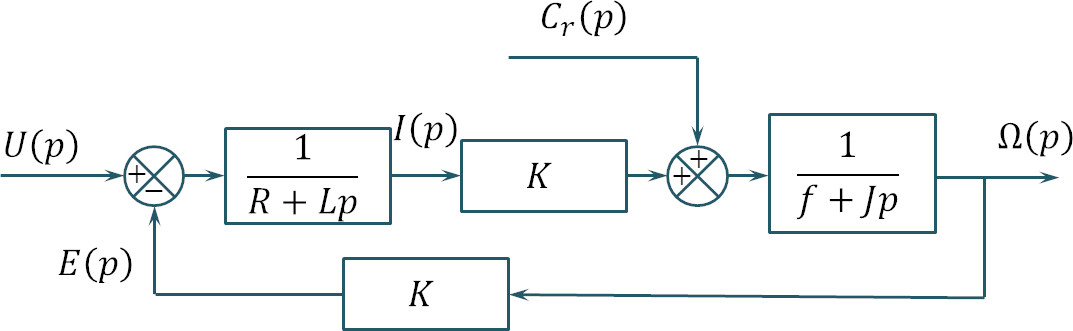
\includegraphics[width=.7\linewidth]{51_01_c}
%\caption{Évolution du couple utile en fonction de la vitesse de rotation pour des
%fréquences de commande de \SI{90}{Hz} à \SI{110}{Hz}. \label{fig_50_04}}
\end{figure}
\else
\fi



\question{Mettre le schéma-blocs sous la forme suivante.}
\ifprof
\begin{figure}[H]
\centering
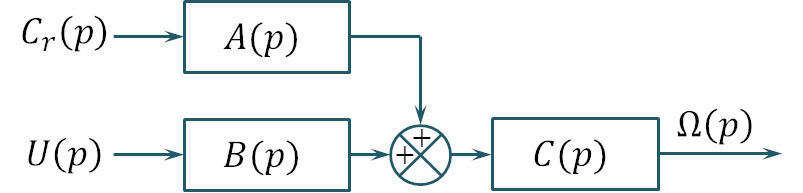
\includegraphics[width=.7\linewidth]{51_01}
%\caption{Évolution du couple utile en fonction de la vitesse de rotation pour des
%fréquences de commande de \SI{90}{Hz} à \SI{110}{Hz}. \label{fig_50_04}}
\end{figure}


En utilisant le schéma-blocs proposé, on a $\Omega(p) = \left(C_r(p)A(p)+U(p)B(p)\right)C(p)$.

D'autre part,  $\Omega(p)=\left( C_r(p) + \dfrac{K}{R+Lp}\left(U(p)-K\Omega(p) \right) \right) \dfrac{1}{f+Jp}$.

On a donc $\left(f+Jp \right)\Omega(p)= C_r(p) + U(p)\dfrac{K}{R+Lp}  $

$\Leftrightarrow \left(f+Jp \right)\Omega(p)+ \dfrac{K^2}{R+Lp}\Omega(p)  = C_r(p) + U(p)\dfrac{K}{R+Lp} $

$\Leftrightarrow \left(\left(f+Jp \right)+ \dfrac{K^2}{R+Lp}\right)\Omega(p)  = C_r(p) + U(p)\dfrac{K}{R+Lp} $

$\Leftrightarrow \dfrac{K^2+\left(f+Jp \right)\left(R+Lp \right)}{R+Lp}\Omega(p)  = C_r(p) + U(p)\dfrac{K}{R+Lp} $

$\Leftrightarrow \Omega(p)  = \left(C_r(p) + U(p)\dfrac{K}{R+Lp}\right)\dfrac{R+Lp}{K^2+\left(f+Jp \right)\left(R+Lp \right)} $.

Dés lors plusieurs schéma-blocs peuvent répondre à la question. Par exemple, $A(p)=1$, $B(p)=\dfrac{K}{R+Lp}$, $C(p)=\dfrac{R+Lp}{K^2+\left(f+Jp \right)\left(R+Lp \right)}$.

En poursuivant, on a aussi : 
$ \Omega(p)  = \left(C_r(p)(R+Lp) + U(p) K\right)\dfrac{1}{K^2+\left(f+Jp \right)\left(R+Lp \right)} $.

On a donc aussi,  $A(p)=R+Lp$, $B(p)={K}$, $C(p)=\dfrac{1}{K^2+\left(f+Jp \right)\left(R+Lp \right)}$



\else
\begin{figure}[H]
\centering
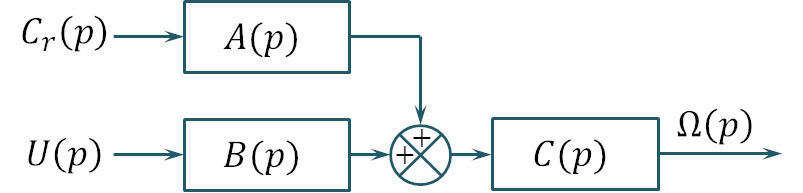
\includegraphics[width=.7\linewidth]{51_01}
%\caption{Évolution du couple utile en fonction de la vitesse de rotation pour des
%fréquences de commande de \SI{90}{Hz} à \SI{110}{Hz}. \label{fig_50_04}}
\end{figure}
\fi





\ifprof
\else

\ifcolle
\else
\noindent\footnotesize
\fbox{\parbox{.9\linewidth}{
Éléments de corrigé : 
\begin{enumerate}
    \item .
    \item $A(p)=R+Lp$, $B(p)={K}$, $C(p)=\dfrac{1}{K^2+\left(f+Jp \right)\left(R+Lp \right)}$ (plusieurs réponses possibles). 
\end{enumerate}}}
\normalsize
\fi
\begin{flushright}
\footnotesize{Corrigé  voir \ref{B2:07:51}.}
\end{flushright}%
\fi